\documentclass[12pt]{article}
\usepackage[utf8]{inputenc}
\usepackage[T2A]{fontenc}
\usepackage[mongolian]{babel}
\usepackage{graphicx}
\usepackage{amsmath}
\usepackage{amssymb}
\graphicspath{{zurag/}}
\begin{document}
	\begin{titlepage}
		\begin{center}
			{\scshape\large Шинжлэх Ухаан Технологийн Их Сургууль\par} %Их сургуулийн нэр
			{\scshape Мэдээлэл, Холбооны Технологийн Сургууль\par}\vspace{0.5cm} %Их сургуулийн нэр
			
			\begin{figure}[!htbp]
				\centering
				
\includegraphics[scale=0.2]{zurag/MUST_logo.png}
			\end{figure}
			
			\vspace{2cm}
			%\hfill \large{} \\
			
			{\huge \bfseries Мэдээллийн системийн төсөл 1\par}\vspace{0.4cm} % Тезисийн нэр
			
			\vspace{2cm}
			
			\begin{minipage}[t] {0.9\textwidth}
				\begin{flushleft} 
					\normalsize
					
					%Мэргэжлийн индекс:  \\
					Мэргэжил: Мэдээллийн систем \\[2cm]
					
					\emph{Удирдагч:} {Т. Золбоо} \\% Удирдагчийн нэр
					%\emph{Зөвлөгч:} {\advicename} \\ % Зөвлөгч нарын нэрс
					\emph{Гүйцэтгэгч:} {Г. Эрдэнэсоёл} \\ % Зохиогчийн нэр
					
				\end{flushleft}
			\end{minipage}
			
			\vfill
			
			{\large  Улаанбаатар хот} \\
			{\large 2018 он}\\ % Date
		\end{center}
	\end{titlepage}
	
	\tableofcontents
	\newpage
	%\listoffigures
	%\newpage
	
	
	
	
	
	\section{Оршил}
	
	Сэтгэгдэл бол агшинаас агшинд үргэлж өөрчлөгдөж байдаг, “ямар нэг зүйл”-ийг туулж мэдрэх бие даасан, субъектив мэдрэмж юм.  Энэ зүйлийг олон нийтийн сүлжээнд хэрхэн яаж илэрхийлэгддэг талаар судалцгаая.
	\section{Зорилго}
	Энэхүү системийн сэтгэгдэл бичих 
	
	\section{Судалгаа}
	Дэлхийн нийтээрээ өдөр тутамд хэрэглэдэг олон нийтийн сүлжээнүүд болох фэйсбүүк, youtube, твиттер, инстаграм гэх мэт сошиал ертөнцөд сэтгэгдлийг цаг, минут тутамд ашигладаг. Жишээ нь фэйсбүүк дээр хэн нэгний зураг, нийтлэл дээр сэтгэгдэл үлдээдэг. Мөн таны нийтлэл дээр хэн нэгэн сэтгэгдэл үлдээж болно. Тэр үед таньд мэдэгдэл ирнэ. Таны нийтлэл дээр үлдээсэн сэтгэгдэл дээр хариу үйлдлүүдийг үзүүлж болно. Сэтгэгдэл үлдээхдээ дан ганц текст хэлбэрээр биш зураг, видео, эможи, хөдөлгөөнт зураг, найзуудаа меншион хийх гэх мэт сэтгэгдэл үлдээдэг. Мөн бичсэн сэтгэгдэлээ засах болон устгаж болдог. Өөрийн болон бусдын сэтгэгдэл дээр хариу үйлдэл үзүүлж болно. Энэ нь таньд таалагдах болон таалагдахгүй байвал эможи хэлбэрээр хариу үйлдэл үзүүлж болно. Өөрийн нийтлэл дээр ирсэн сэтгэгдэлийг ч мөн нуух болон устгаж болдог. Нийтлэл бичсэн хүн нийтлэлээ устгасан тохиолдолд таны үлдээсэн сэтгэгдэл устна. Үүнтэй адил " Их сургуулийн олон нийтийн сүлжээний систем"ийн сэтгэгдэл үлдээх хэсэг нь хэрэглэгч ямар нэгэн хүний нийтлэл доор өөрийн санаа бодлыг энгийн текстээр болон зураг, хөдөлгөөнт зураг, эможи, файл гэх мэтээр үлдээх явдал юм. Нийтлэл нь текст, зураг гэх мэт өөр өөр байж болно. 
	\section{Бизнес процессийн диаграм}
	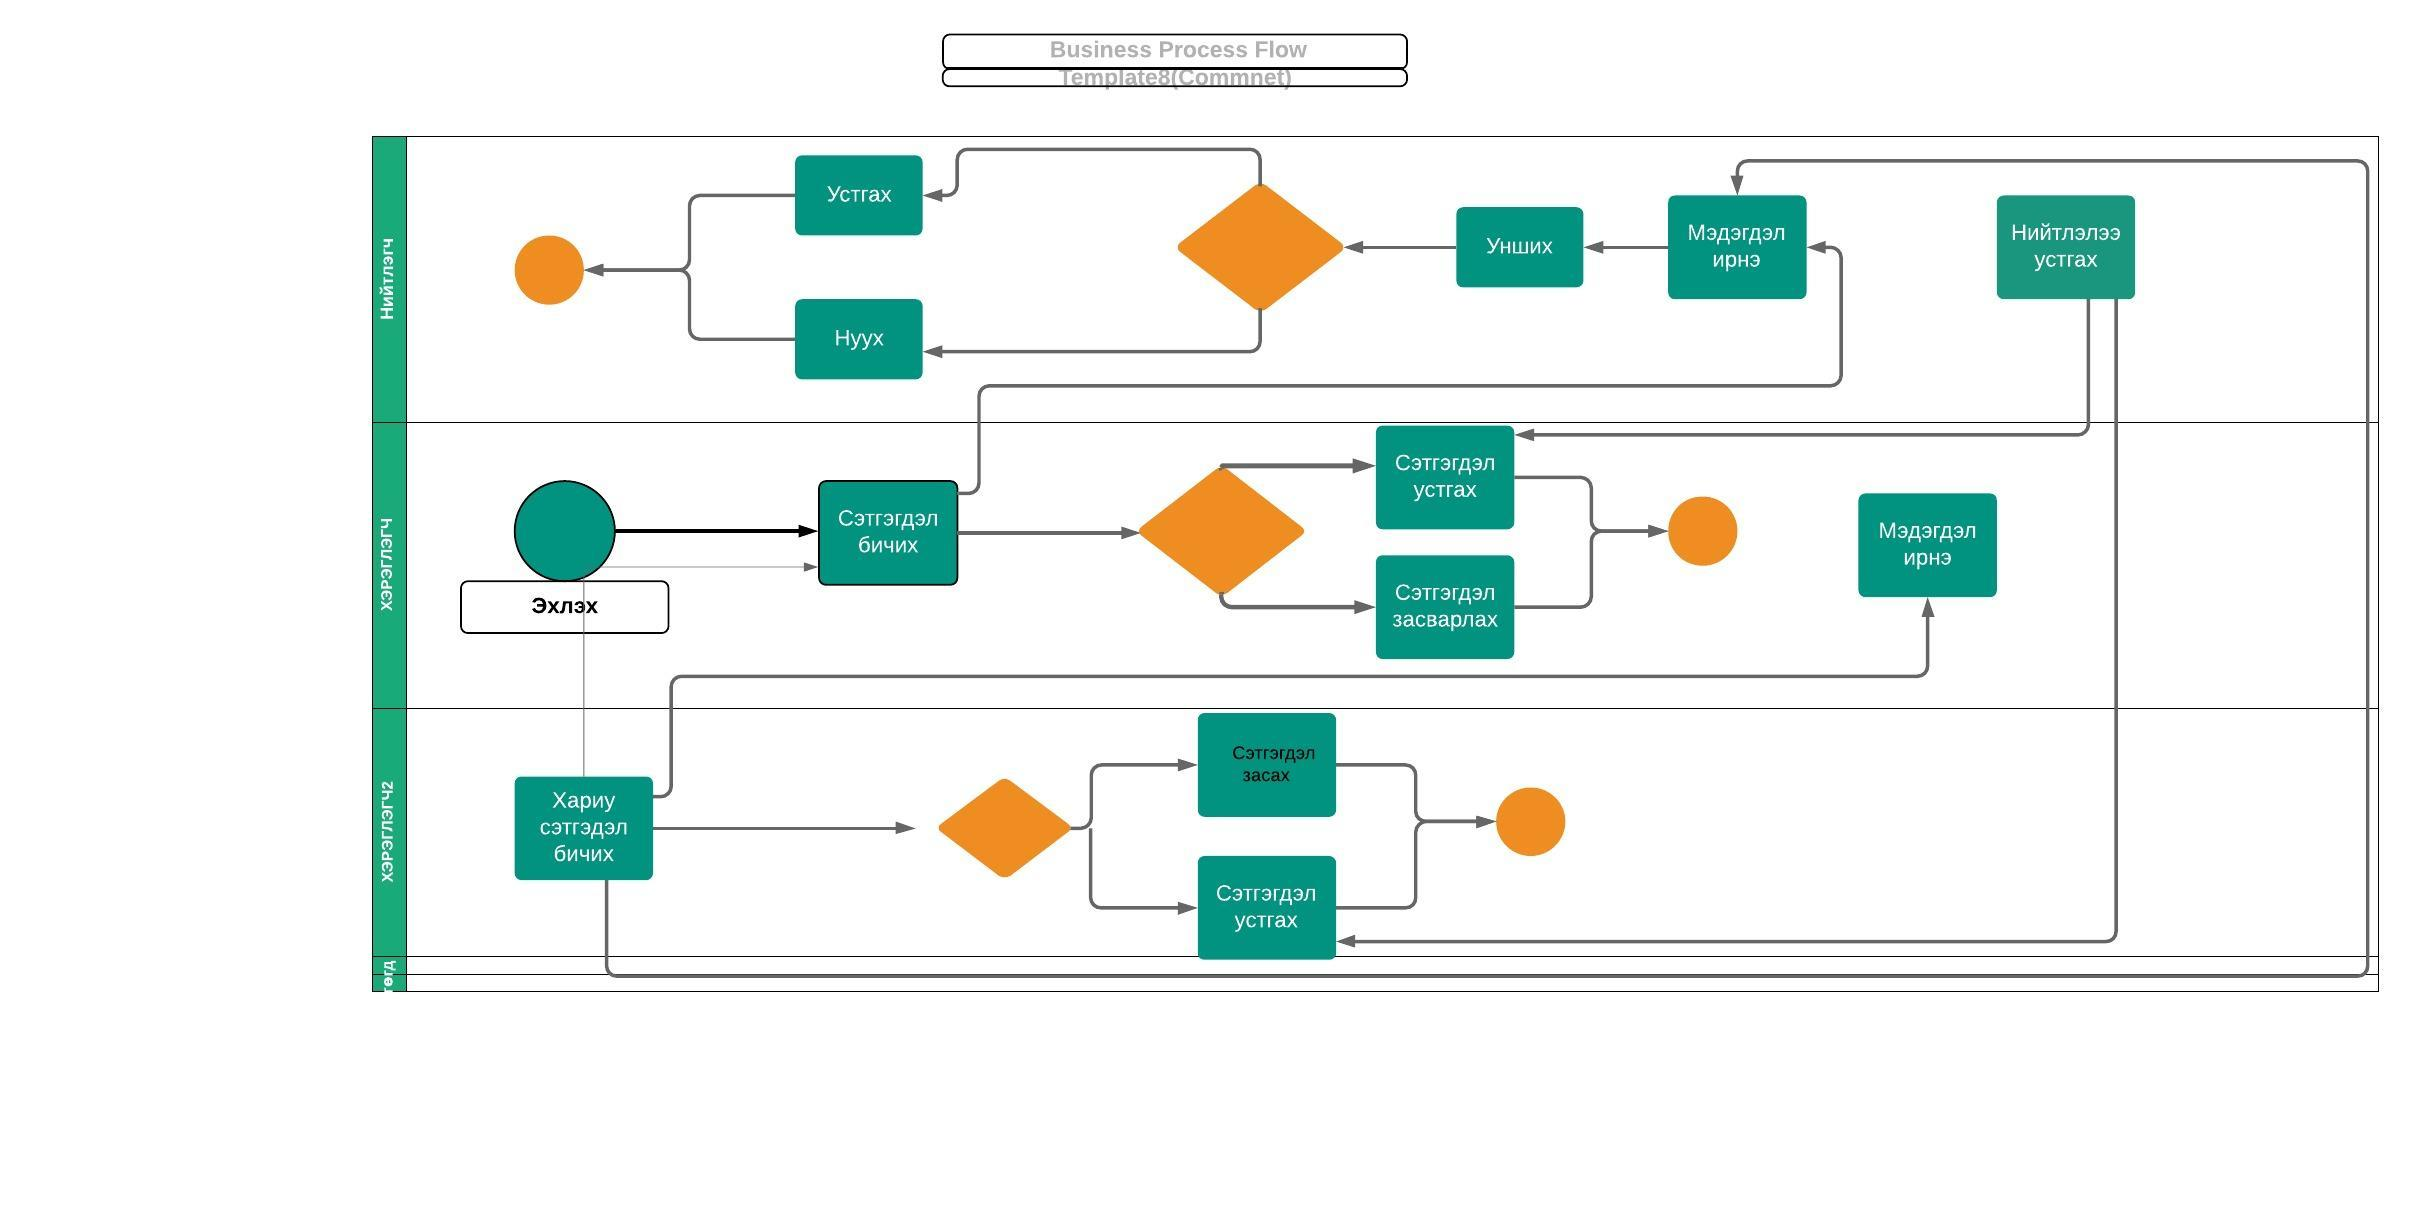
\includegraphics[scale=0.5]{BPDiagram} 
	\section{Судалсан систем}
	\begin{itemize}
		\item фэйсбүүк
		\item инстаграм
		\section{Функциональ шаардлага}	
		\begin{itemize}
			\item Сэтгэгдэл нь давтагдашгүй дугаартай байх.
			\item Хэрэглэгчийн хариу бичсэн сэтгэгдэл болгон давтагдашгүй дугаартай байх.(ParentComment).
			\item Нийтлэлд харгалзах бүх сэтгэгдэлүүдийг харж болдог байх
			\item Бусдын сэтгэгдэл дээр Like, Dislike, Emoji дардаг байх.
			\item Тухайн хүн өөрийнх нь сэтгэгдэл болон, бусдын сэтгэгдэл дээр Like, DisLike, Emoji дарсан хүмүүсийн тоо, тэдгээрийн нэрсийн жагсаалтыг харах боломжтой байх.
			\item Сэтгэгдэл талбарт бусад хэрэглэгчийн нэрийг бичиж мэдэгдэл өгдөг байх. 
			\item Сэтгэгдэл талбар дээр (Тухайн URL-ийн Preview) оруулж хийхэд Веб сайтын гарчиг, тайлбар, thumb гарч ирдэг байх.
			\item Сэтгэгдэл хэдний өдөр хэдэн цагт бичсэнийг харуулдаг байх.
			\item Зурагтай сэтгэгдэл/сэтгэгдэлд зураг хавсаргаж оруулж болдог байх.
			\item Өөрийн бичсэн сэтгэгдлийг засаж, устгаж болдог байх.
			\item Хүн бүр хүссэн хүний сэтгэгдлийг Report хийж мэдэгддэг байх.
		\end{itemize}
		
		
		
		\section{Функциональ бус шаардлага}
		\begin{itemize}
			\item Сэтгэгдэл бичих тоо 300-аас хэтрэхгүй байх.
			\item Нэг хүн хэдэн ч сэтгэгдэл үлдээж болдог байх.
			\item Нэг хүн нэг нийтлэлд дараалж 5-аас ихгүй сэтгэгдэл үлдээдэг байх.
			\item Сэтгэгдэлийг шүүж оруулдаг байх(хараалын үг, доромж үг)
			\item Зүй бус үг хэллэг орсон байвал сэтгэгдэл үлдээлгэхгүй байх эсвэл доромжилсон үгийг дарж оруулдаг байх.
			\item Parent Сэтгэгдэл нь 1-ээс ихгүй үүсдэг байх.
		\end{itemize}
	\end{itemize}
	
	\section{Use case диаграм}
	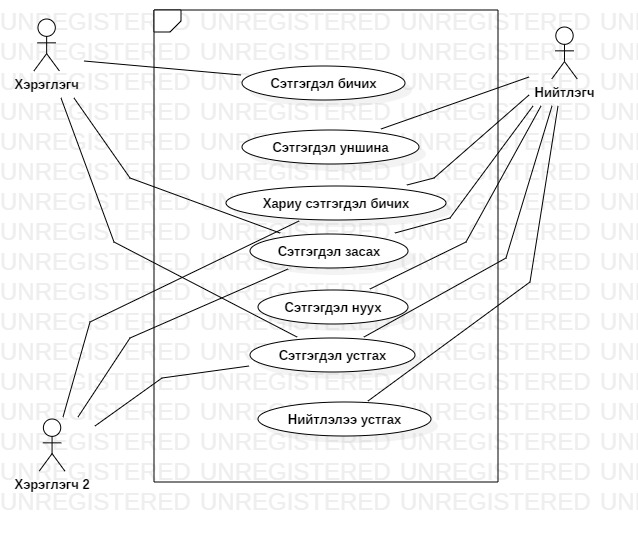
\includegraphics[scale=0.5]{UseCaseDiagram} 
	
	\section{Класс диаграм}
	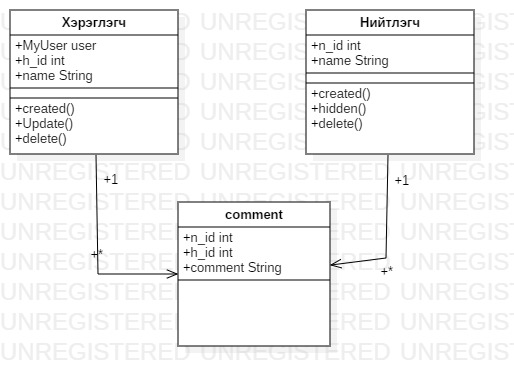
\includegraphics[scale=0.5]{commentclass} 
	
	\section{Дарааллын диаграм}
	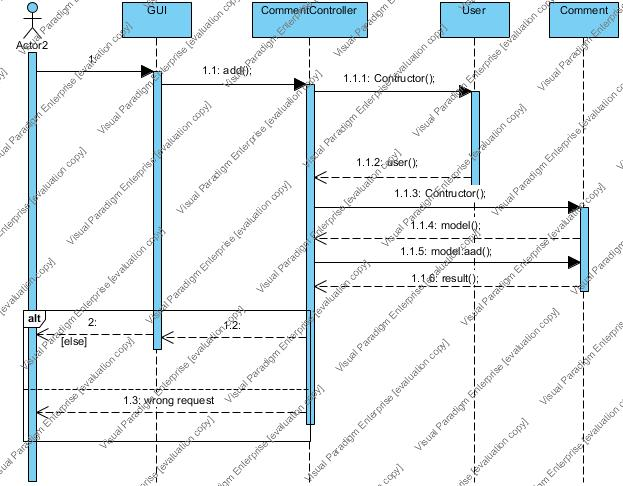
\includegraphics[scale=0.5]{Sequence01} 
	
	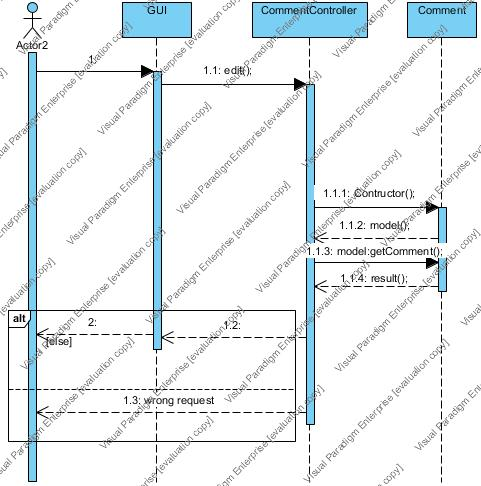
\includegraphics[scale=0.5]{Sequence02} 
	
	
	\section{Activity диаграм}
	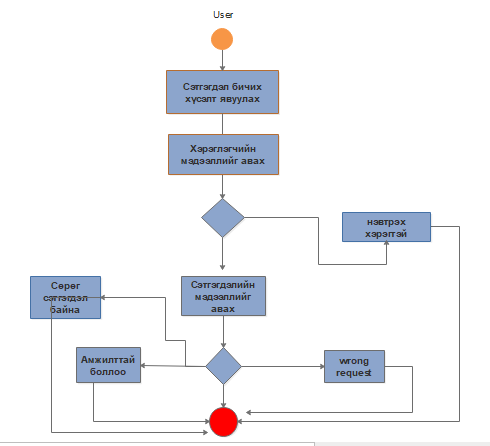
\includegraphics[scale=0.5]{Activity1} 
	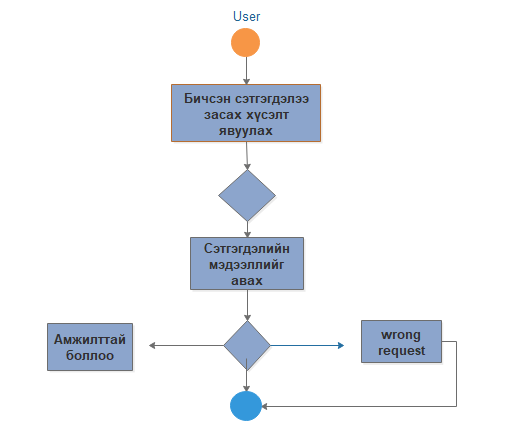
\includegraphics[scale=0.5]{Activity2} 
	
	\section{Ажлын урсгалын диаграм}
	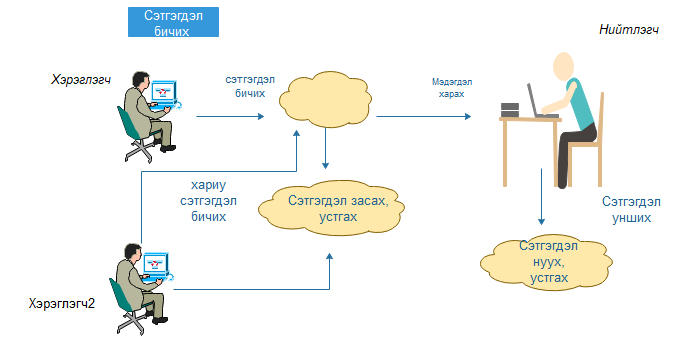
\includegraphics[scale=0.5]{workflow2}
	\section{Дэлгэцийн зохиомж}
	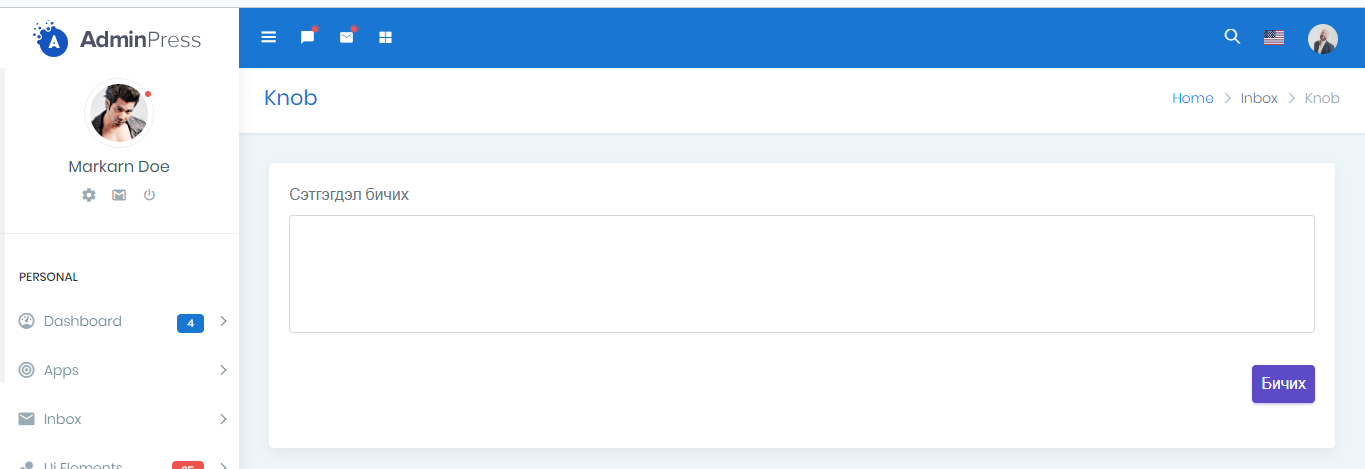
\includegraphics[scale=0.5]{comment1}
	
	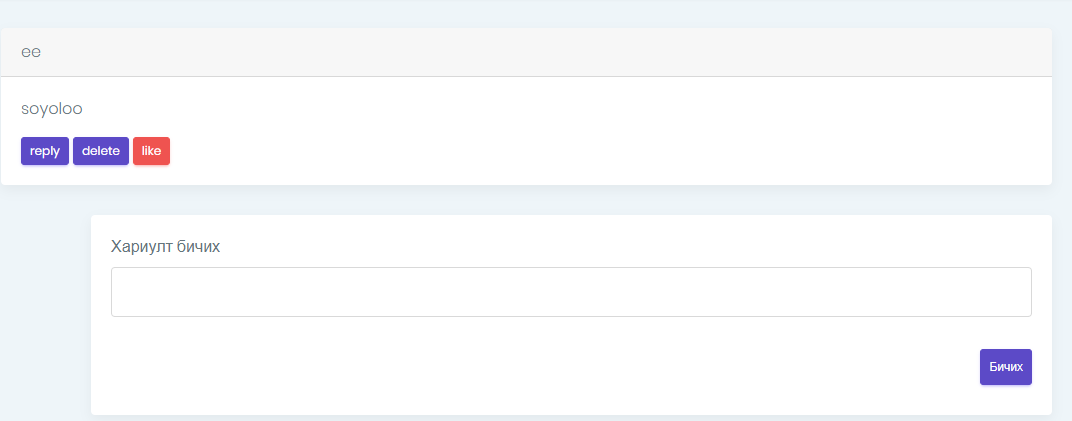
\includegraphics[scale=0.5]{comment3}
	
	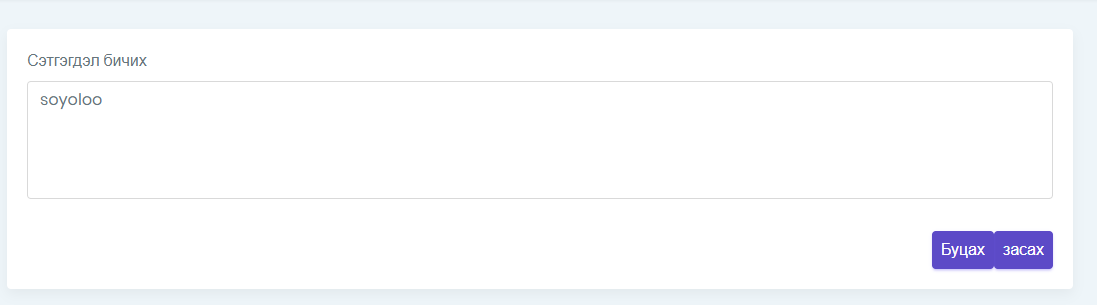
\includegraphics[scale=0.5]{comment4}
	
	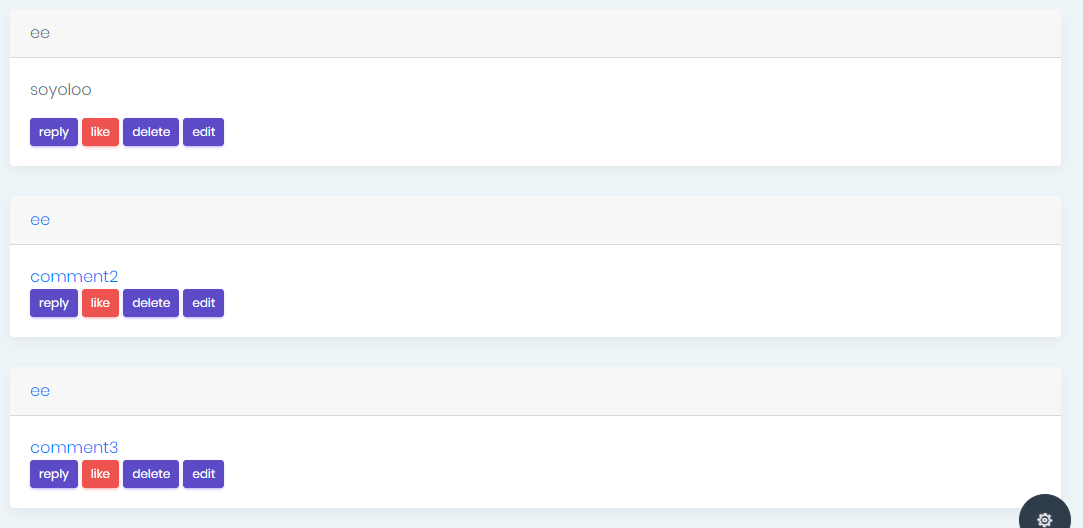
\includegraphics[scale=0.5]{comment5}
		\section{Тест}
	
	
	\section{Дүгнэлт}
	\begin{itemize}
		Энэхүү системийн сэтгэгдлийн хэсгийг судалгаа дээр үндэслэн хийсэн. Сэтгэгдэл үлдээх хэсгэн дээр системийн хэрэглэгч сэтгэгдэл үлдээх боломжтой болсон. Ингэснээр хэрэглэгч дурын нийтлэл дээр өөрийн үзэл илэрхийлэх хэн нэгний сэтгэгдэлд хариулах гэм мэт үйлдлүүдийг хийх юм. 
		hjgjhghh
		
	\end{itemize}
	
	
	
	
\end{document}